%!TEX root = informe.tex
\chapter{Introducción}
\section{Antecedentes}

La mayoría de las ciudades europeas utilizan materiales prefabricados basados en el cemento para urbanizar el terreno transformándolo en espacio público que utilizarán los ciudadanos. Estas instalaciones deben ser resistentes, económicas, funcionales y sobre todo sostenibles. La sostenibilidad es un requisito que ha ido ganando importancia en los últimos años debido no solo al aspecto económico —costes y mantenimiento principalmente— sino también al medioambiental.

El impacto medioambietal que producen las actividades humanas en la naturaleza debería convertirse en un elemento más de estudio en cualquier proyecto de ingeniería actual. En el caso de este proyecto, el sector de las obras civiles y urbanismo supone un consumo muy elevado de materias primas y energía debido a que representa un porcentaje importante de la actividad económica de cualquier país occidental, lo que implica altas emisiones al medio ambiente. De esta manera, utilizando la metodología del Análisis de Ciclo de Vida (ACV) se pretende conocer con una rigurosidad adecuada el ciclo de vida de un producto y/o servicio, evaluando el impacto potencial sobre el medio ambiente a lo largo de su vida.

% El ecodiseño se define como la incorporación de criterios ambientales en la fase de diseño de un producto o servicio. Surge como respuesta a la necesidad de introducir criterios ambientales durante todo el ciclo de vida de cualquier producto con el objetivo de prevenir o reducir su impacto ambiental.
% El ecodiseño incorpora criterios ambientales en la fase de diseño para minimizar los residuos, las emisiones y los costes energéticos así como los recursos en general.
% En este sentido, la norma UNE_EN ISO 14006:2011 proporciona las directrices para ayudar a las organizaciones a integrar el ecodiseño como parte de un sistema de gestión (SG).

\section{Objetivos y alcance}
El objetivo principal de este proyecto es el Análisis de Ciclo de Vida de un adoquín común utilizado en obras civiles y urbanismo. Se pretende analizar todas las entradas y salidas tanto de materiales como de energía desde la extracción de la materia prima hasta el final de vida del producto, además de identificar y clasificar los principales aspectos medioambientales y sus correspondientes impactos en los diferentes procesos que intervienen en su fabricación. De esta forma, se pueden establecer los siguientes objetivos básicos:
\begin{itemize}
\item análisis del ciclo de vida del proceso de fabricación, desde la extracción de las materias primas hasta que se obtiene el producto en fábrica.
\item análisis del ciclo de vida de la instalación del producto, desde que sale de la fábrica hasta que se encuentra en su lugar de destino.
\item análisis del ciclo de vida del uso y mantenimiento del producto, desde que se empieza a utilizar hasta que se decide retirar.
\item análisis del ciclo de vida del final de vida del producto, desde que es retirado hasta que se convierte en residuos o en nuevos productos.
\end{itemize}

A su vez, la redacción del presente proyecto bajo la dirección del Departamento de Expresión Gráfica, Diseño y Proyectos de la Universidad de Málaga tiene como finalidad última la obtención del título de Ingeniero Industrial.

\section{Metodología}

El presente proyecto seguirá el siguiente proceso de estudio:

\begin{itemize}
  \item En primer lugar se establecen las características del producto a estudio, historia de su desarrollo y materias primas que lo componen.
  \item Se expondrá la relevancia del producto con el impacto medioambiental y se explicará la metodología de Análisis de Ciclo de Vida, su importancia y las herramientas con las que se trabajará.
  \item A continuación se realizará un Análisis de Ciclo de Vida del producto desde ``la cuna hasta la tumba'', es decir: extracción de materias primas, fabricación, instalación, uso y mantenimiento, y fin de vida.
  \item Una vez analizados, se hará una comparación entre ellos.
  \item Por último, se desarrollarán las conclusiones obtenidas del estudio y posibles mejoras o futuras líneas de expansión.
\end{itemize}

\section{Origen del estudio}
Malaka de Prefabricados es una empresa malagueña que inició su actividad en 1994. Su compromiso consistía en integrarse en el tejido industrial de la provincia, estableciendo lazos con otras industrias locales, y apostar por un producto de calidad que marcara la diferencia en el mercado sin repercutir en el precio.

\begin{figure}[!htb]
\centering
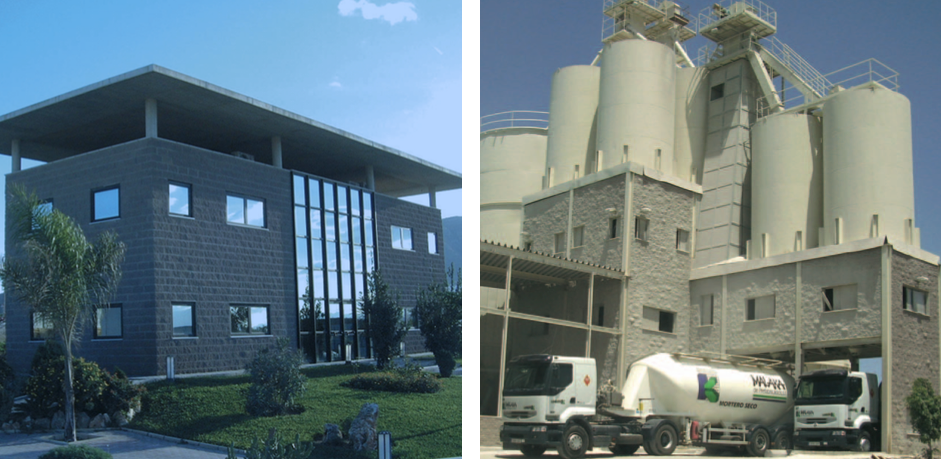
\includegraphics[width=15cm]{malaka1.png}
\caption[Instalaciones de Malaka de Prefabricados.]{Instalaciones de Malaka de Prefabricados. Fuente: \protect\cite{malakacatalogo}.}
\label{fig:malakainstalaciones1}
\end{figure}

A finales de la década de los 90 y principios del nuevo milenio experimentaron un fuerte crecimiento como consecuencia del rápido auge del sector de la construcción en Andalucía, convirtiéndose en un referente de los prefabricados en la provincia y en la comunidad autónoma.

Sus principales líneas de producción son los adoquines, bloques y bordillos de hormigón, a los que se dedica por completo una planta de producción automatizada. La línea de adoquines dispone de varias gamas de producto debido a la versatilidad y demanda de la que disfruta. El resto de productos —tubos, registros, aligerantes, casetones y mortero seco ensilado— se fabrican en la segunda planta.

\begin{figure}[!htb]
\centering
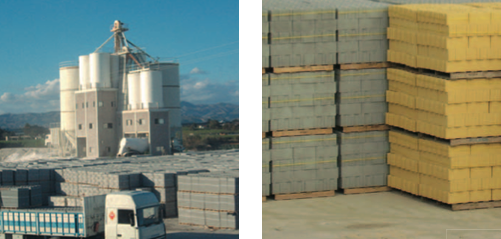
\includegraphics[width=15cm]{malaka2.png}
\caption[Instalaciones accesorias de Malaka de Prefabricados.]{Instalaciones accesorias de Malaka de Prefabricados. Fuente: \protect\cite{malakacatalogo}.}
\label{fig:malakainstalaciones2}
\end{figure}

El compromiso de calidad en sus productos pasó por cumplir todos los requisitos de la normativa española y europea, adoptando el marcado CE como sello de calidad. Tanto clientes como partners pueden dar muestra de su confianza en la calidad de los mismos. Entre sus principales proyectos se encuentran el Palacio de Deportes Martín Carpena (Ferrovial—Agroman), el Parque Temático de Melilla (Dragados) y colaboraciones con los ayuntamientos de Marbella y Estepona.

Durante los casi veinte años en la industria han intentado adoptar las mejores y más novedosas tecnologías de fabricación del sector, ampliando de forma progresiva el tamaño de sus instalaciones en la Finca Pizarro, a las afueras de la ciudad de Málaga.

La empresa adoptó a principios de 2000 la Certificación de Sistemas de Gestión de la Calidad (ISO 9001) y varios años más tarde la Certificación Sistemas de Gestión Ambiental (ISO 14000) como referente de compromiso con la calidad de su producción y con el medioambiente.
